\documentclass[12pt]{article}
\usepackage{graphicx}
\usepackage{float}
\usepackage{hyperref}
\usepackage[brazil]{babel}
\usepackage[utf8]{inputenc}
\usepackage{amsmath}
\usepackage{geometry}

\geometry{a4paper, margin=1in}

% Informações do trabalho
\title{Análise de Desempenho}
\author{Antonio Neto}
\date{2024}

\begin{document}

\maketitle

\begin{abstract}
 Este relatório tem como objetivo explorar os conceitos de análise de desempenho de algoritmos, utilizando ferramentas como \textit{time} e \textit{perf} em uma distribuição Ubuntu 20.04, tanto em container quanto em virtualização. O estudo foca na implementação de algoritmos para cálculo do fatorial de um número, utilizando métodos recursivo e iterativo, bem como na comparação de desempenho entre eles. Adicionalmente, foram analisados algoritmos de divisão e operações de escrita em arquivo. \textbf{O DockerRun.txt} tem os dados brutos da execução do container, e os comandos utilizados podem ser encontrados no  \textbf{README.md}. Códigos do container estão no \textbf{DockerFile}, com uma implementação bem sucedida do \textit{perf} mesmo usando WSL2. Também executei o script no VirtualBox, mas a diferença não foi muito grande comparada ao container; os resultados estão em \textbf{LinuxTerminal.txt} apenas para demonstração.
\end{abstract}

\tableofcontents

\newpage

\section{Desenvolvimento}
Os experimentos foram realizados em um container Docker. Os códigos em C foram desenvolvidos para calcular o fatorial de 10,20,30,40,50,60,70,80,90 e 100 de forma recursiva e iterativa, realizar operações de divisão de inteiros e floats, e operações de escrita em arquivo. Scripts em Python foram utilizados para automatizar a execução dos testes, coletar e analisar os dados, e gerar gráficos comparativos. Vale mencionar que os scripts para calcular o fatorial não são convencionais, pois utilizei vetores para armazenar os dígitos do resultado, permitindo calcular fatoriais de números que usariam bem mais de 64 bits. Também é preciso considerar que os códigos estão sendo executados em ambiente virtualizado, e não refletem a realidade de modo absoluto!

\subsection{Implementação dos Algoritmos}
Os algoritmos foram implementados conforme descrito abaixo:

\subsubsection{Algoritmo Recursivo}
\begin{verbatim}
#include <stdio.h>
#include <stdlib.h>
#include <string.h>

#define MAX_DIGITS 5000

void multiply(int result[], int *result_size, int x) {
    int carry = 0;
    for (int i = 0; i < *result_size; ++i) {
        int prod = result[i] * x + carry;
        result[i] = prod % 10;
        carry = prod / 10;
    }

    while (carry) {
        result[(*result_size)++] = carry % 10;
        carry /= 10;
    }
}

void factorial_recursive(int result[], int *result_size, int n) {
    if (n == 1) {
        return;
    }

    factorial_recursive(result, result_size, n - 1);
    multiply(result, result_size, n);
}

void print_result(int result[], int result_size) {
    for (int i = result_size - 1; i >= 0; --i) {
        printf("%d", result[i]);
    }
    printf("\n");
}

int main(int argc, char *argv[]) {
    if (argc != 2) {
        printf("Usage: %s <number>\n", argv[0]);
        return 1;
    }

    int num = atoi(argv[1]);
    if (num < 0) {
        printf("Please enter a non-negative integer.\n");
        return 1;
    }

    int result[MAX_DIGITS];
    memset(result, 0, sizeof(result));
    result[0] = 1;
    int result_size = 1;

    factorial_recursive(result, &result_size, num);

    print_result(result, result_size);

    return 0;
}
\end{verbatim}

\subsubsection{Algoritmo Iterativo}
\begin{verbatim}
#include <stdio.h>
#include <stdlib.h>
#include <string.h>

#define MAX_DIGITS 5000

void multiply(int result[], int *result_size, int x) {
    int carry = 0;
    for (int i = 0; i < *result_size; ++i) {
        int prod = result[i] * x + carry;
        result[i] = prod % 10;
        carry = prod / 10;
    }

    while (carry) {
        result[(*result_size)++] = carry % 10;
        carry /= 10;
    }
}

void factorial_iterative(int result[], int *result_size, int n) {
    for (int x = 2; x <= n; ++x) {
        multiply(result, result_size, x);
    }
}

void print_result(int result[], int result_size) {
    for (int i = result_size - 1; i >= 0; --i) {
        printf("%d", result[i]);
    }
    printf("\n");
}

int main(int argc, char *argv[]) {
    if (argc != 2) {
        printf("Usage: %s <number>\n", argv[0]);
        return 1;
    }

    int num = atoi(argv[1]);
    if (num < 0) {
        printf("Please enter a non-negative integer.\n");
        return 1;
    }

    int result[MAX_DIGITS];
    memset(result, 0, sizeof(result));
    result[0] = 1;
    int result_size = 1;

    factorial_iterative(result, &result_size, num);

    print_result(result, result_size);

    return 0;
}
\end{verbatim}

\newpage

Gráfico representando o comando time executado nos códigos de fatorial. Demonstrou ser pouco preciso.

\begin{figure}[H]
    \centering
    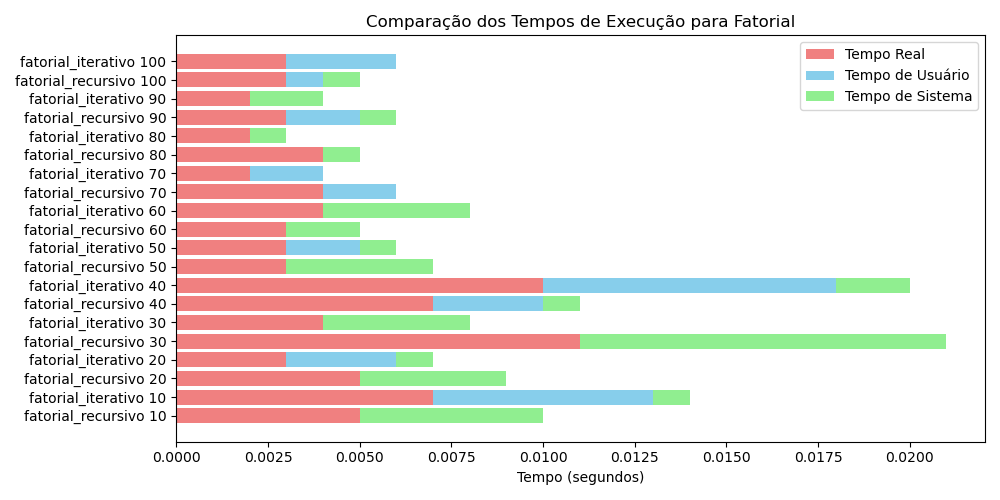
\includegraphics[width=\linewidth]{./resultados/time_fatorial.png}
    \caption{Tempo de Execução dos Algoritmos de Fatorial (time)}
    \label{fig:time_fatorial}
\end{figure}

\subsubsection{Divisão de Inteiros}
\begin{verbatim}
#include <stdio.h>

int main() {
    for (int i = 1; i <= 1000000; ++i) {
        int a = i, b = i + 1;
        int c = a / b;
        int d = b / a;
        int e = a / a;
        int f = b / b;
    }
    return 0;
}
\end{verbatim}

\subsubsection{Divisão de Floats}
\begin{verbatim}
#include <stdio.h>

int main() {
    for (int i = 1; i <= 1000000; ++i) {
        float a = (float)i, b = (float)(i + 1);
        float c = a / b;
        float d = b / a;
        float e = a / a;
        float f = b / b;
    }
    return 0;
}
\end{verbatim}

\subsubsection{Operações de Escrita em Arquivo}
\begin{verbatim}
#include <stdio.h>

int main() {
    FILE *file = fopen("output.txt", "w");
    if (!file) {
        perror("Erro ao abrir o arquivo");
        return 1;
    }

    for (int i = 1; i <= 1000000; ++i) {
        int a = i, b = i + 1;
        int c = a / b;
        fprintf(file, "%d\n", c);
    }

    fclose(file);
    return 0;
}
\end{verbatim}

\subsection{Execução dos Testes}
Os testes foram realizados para entradas variando de 10 a 100 no caso dos algoritmos de fatorial, e para um loop de 1 a 1 milhão nos casos das divisões e operações de escrita. As ferramentas \textit{time} e \textit{perf} foram utilizadas para medir o tempo de execução e coletar métricas de desempenho. O script \textit{run\_tests.sh} foi utilizado para automatizar a execução dos testes e salvar os resultados.

\subsection{Coleta e Análise dos Dados}
Os resultados dos testes foram organizados no arquivo \textbf{DockerRun.json}, que foi posteriormente analisado utilizando o plot.py. Este script utilizou a biblioteca \textit{matplotlib} para gerar gráficos comparativos dos tempos de execução e outras métricas de desempenho:

\begin{verbatim}
import json
import matplotlib.pyplot as plt
import numpy as np
import os
import re

if not os.path.exists('resultados'):
    os.makedirs('resultados')

with open('DockerRun.json') as f:
    data = json.load(f)

executions = data['executions']
metrics = ['task_clock', 'cycles', 'instructions', 'branches', 'branch_misses', 'l1_dcache_loads', 'l1_dcache_load_misses']

metrics_data = {metric: [] for metric in metrics}
names = []
real_times = []
user_times = []
sys_times = []

def parse_time(time_str):
    # Extract only the numeric part and convert it to float
    return float(re.findall(r"[-+]?\d*\.\d+|\d+", time_str)[0])

for execution in executions:
    names.append(f"{execution['name']} {execution.get('input', '')}".strip())
    real_time_str = execution['real_time']
    user_time_str = execution['user_time']
    sys_time_str = execution['sys_time']
    real_times.append(parse_time(real_time_str)) 
    user_times.append(parse_time(user_time_str)) 
    sys_times.append(parse_time(sys_time_str))   
    for metric in metrics:
        value_str = execution['perf_output'].get(metric, '0')
        value = float(value_str.split()[0].replace(',', ''))
        metrics_data[metric].append(value)

metric_translations = {
    'task_clock': 'Tempo de Tarefa',
    'cycles': 'Ciclos',
    'instructions': 'Instruções',
    'branches': 'Ramificações',
    'branch_misses': 'Falhas de Ramificação',
    'l1_dcache_loads': 'Carregamentos L1 DCache',
    'l1_dcache_load_misses': 'Falhas de Carregamento L1 DCache'
}

# Cálculo das métricas adicionais
def calculate_metrics(execution, real_time, user_time, sys_time):
    instructions = float(execution['perf_output']['instructions'].split()[0].replace(',', ''))
    cycles = float(execution['perf_output']['cycles'].split()[0].replace(',', ''))
    
    # Assumindo frequência do clock em Hz (ex: 2.5GHz = 2.5 * 10^9 Hz)
    clock_frequency = 2.5 * 10**9 
    
    # Tempo de CPU
    cpu_time = cycles / clock_frequency

    # Percentual do tempo total gasto pela CPU no programa
    total_cpu_time = user_time + sys_time
    percent_cpu_time = total_cpu_time / real_time

    # MIPS
    mips = (instructions / total_cpu_time) / 10**6

    # Assumindo um número fictício de operações de ponto flutuante
    floating_point_operations = 10**6 
    mflops = (floating_point_operations / total_cpu_time) / 10**6

    # Performance
    performance = 1 / real_time

    return percent_cpu_time, mips, mflops, cpu_time, performance

# Calcular e exibir métricas para cada execução
for i, execution in enumerate(executions):
    real_time = real_times[i]
    user_time = user_times[i]
    sys_time = sys_times[i]
    percent_cpu_time, mips, mflops, cpu_time, performance = calculate_metrics(execution, real_time, user_time, sys_time)

    print(f"Métricas para {names[i]}:")
    print(f"Percentual do tempo total gasto pela CPU: {percent_cpu_time:.2f}")
    print(f"MIPS: {mips:.2f}")
    print(f"MFLOPS: {mflops:.2f}")
    print(f"Tempo de CPU: {cpu_time:.6f} segundos")
    print(f"Performance: {performance:.6f}")
    print()

factorial_indices = [i for i, name in enumerate(names) if 'fatorial' in name]
other_indices = [i for i, name in enumerate(names) if 'fatorial' not in name]

factorial_names = [names[i] for i in factorial_indices]
factorial_real_times = [real_times[i] for i in factorial_indices]
factorial_user_times = [user_times[i] for i in factorial_indices]
factorial_sys_times = [sys_times[i] for i in factorial_indices]

other_names = [names[i] for i in other_indices]
other_real_times = [real_times[i] for i in other_indices]
other_user_times = [user_times[i] for i in other_indices]
other_sys_times = [sys_times[i] for i in other_indices]

plt.figure(figsize=(10, 5))
plt.barh(factorial_names, factorial_real_times, color='lightcoral', label='Tempo Real')
plt.barh(factorial_names, factorial_user_times, color='skyblue', label='Tempo de Usuário', left=np.array(factorial_real_times))
plt.barh(factorial_names, factorial_sys_times, color='lightgreen', label='Tempo de Sistema', left=np.array(factorial_real_times) + np.array(factorial_user_times))
plt.xlabel('Tempo (segundos)')
plt.title('Comparação dos Tempos de Execução para Fatorial')
plt.legend()
plt.tight_layout()
plt.savefig('resultados/tempo_execucao_fatorial.png')
plt.close()

plt.figure(figsize=(10, 5))
plt.barh(other_names, other_real_times, color='lightcoral', label='Tempo Real')
plt.barh(other_names, other_user_times, color='skyblue', label='Tempo de Usuário', left=np.array(other_real_times))
plt.barh(other_names, other_sys_times, color='lightgreen', label='Tempo de Sistema', left=np.array(other_real_times) + np.array(other_user_times))
plt.xlabel('Tempo (segundos)')
plt.title('Comparação dos Tempos de Execução para Outras Funções')
plt.legend()
plt.tight_layout()
plt.savefig('resultados/tempo_execucao_outras.png')
plt.close()

for metric, values in metrics_data.items():
    plt.figure(figsize=(10, 5))
    plt.barh(names, values, color='skyblue')
    plt.xlabel(metric_translations[metric])
    plt.title(f'Comparação de {metric_translations[metric]} entre Execuções')
    plt.tight_layout()
    plt.savefig(f'resultados/{metric}.png')
    plt.close()

\end{verbatim}

\newpage

\section{Resultados e Discussão}
Os gráficos a seguir apresentam os tempos de execução dos algoritmos recursivo e iterativo para o cálculo do fatorial, bem como métricas de desempenho coletadas com a ferramenta \textit{perf}.

\begin{figure}[H]
    \centering
    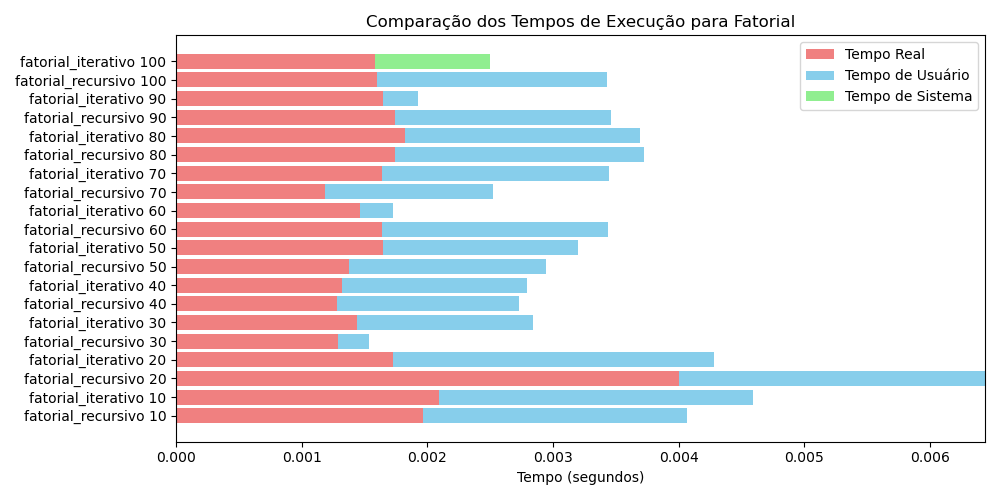
\includegraphics[width=\linewidth]{resultados/tempo_execucao_fatorial.png}
    \caption{Tempo de Execução dos Algoritmos de Fatorial (perf)}
    \label{fig:tempo_execucao}
\end{figure}

\begin{figure}[H]
    \centering
    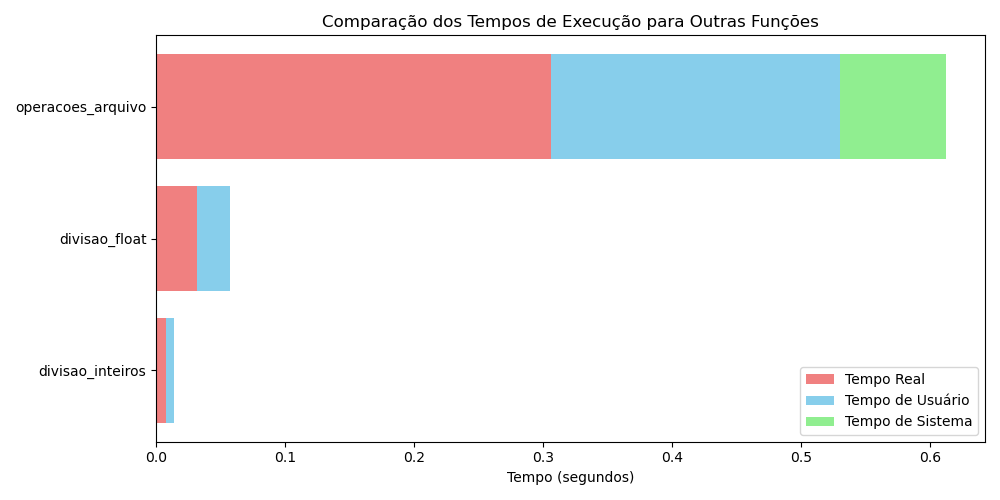
\includegraphics[width=\linewidth]{resultados/tempo_execucao_outras.png}
    \caption{Tempo de Execução de Outras Funções}
    \label{fig:tempo_execucao_outras}
\end{figure}

\begin{figure}[H]
    \centering
    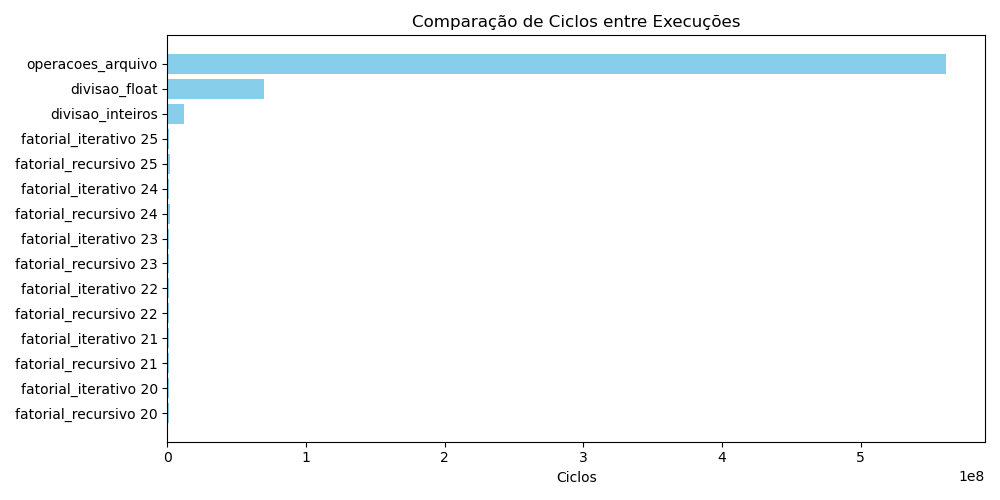
\includegraphics[width=\linewidth]{resultados/cycles.png}
    \caption{Ciclos de CPU dos Algoritmos}
    \label{fig:ciclos_cpu}
\end{figure}

\begin{figure}[H]
    \centering
    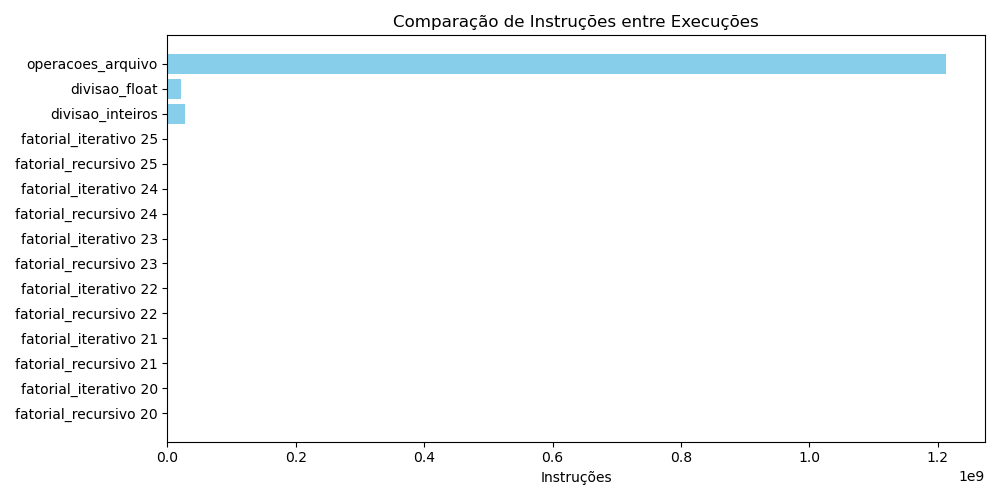
\includegraphics[width=\linewidth]{resultados/instructions.png}
    \caption{Instruções de CPU dos Algoritmos}
    \label{fig:instrucoes_cpu}
\end{figure}

\begin{figure}[H]
    \centering
    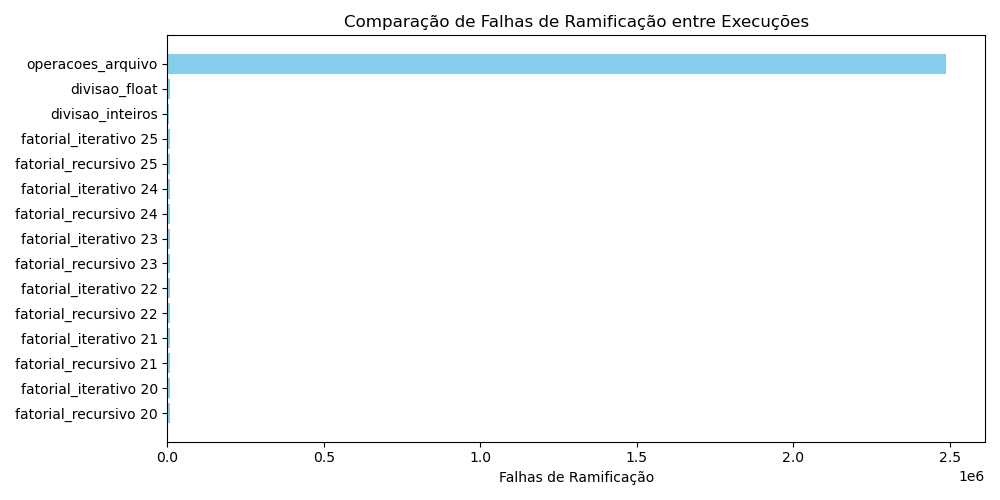
\includegraphics[width=\linewidth]{resultados/branch_misses.png}
    \caption{Branch Misses dos Algoritmos}
    \label{fig:branch_misses}
\end{figure}

\begin{figure}[H]
    \centering
    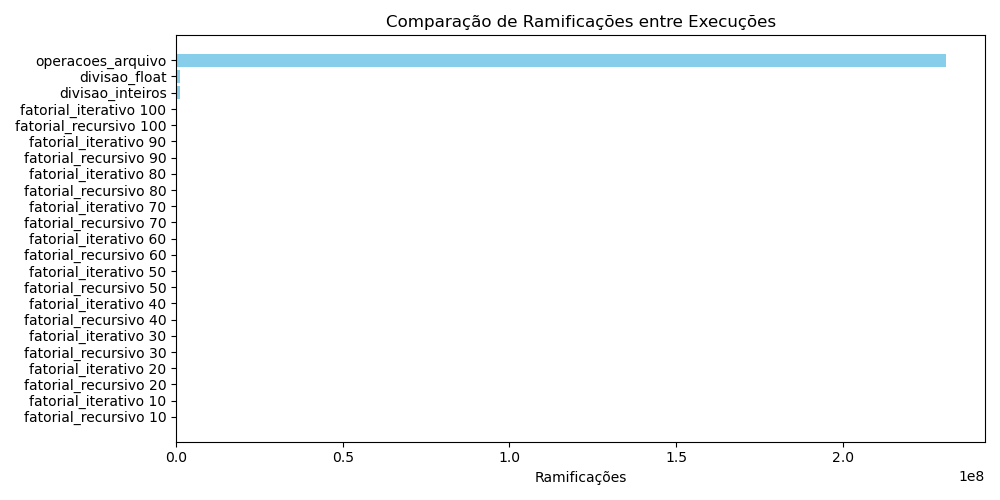
\includegraphics[width=\linewidth]{resultados/branches.png}
    \caption{Branches dos Algoritmos}
    \label{fig:branches}
\end{figure}

\begin{figure}[H]
    \centering
    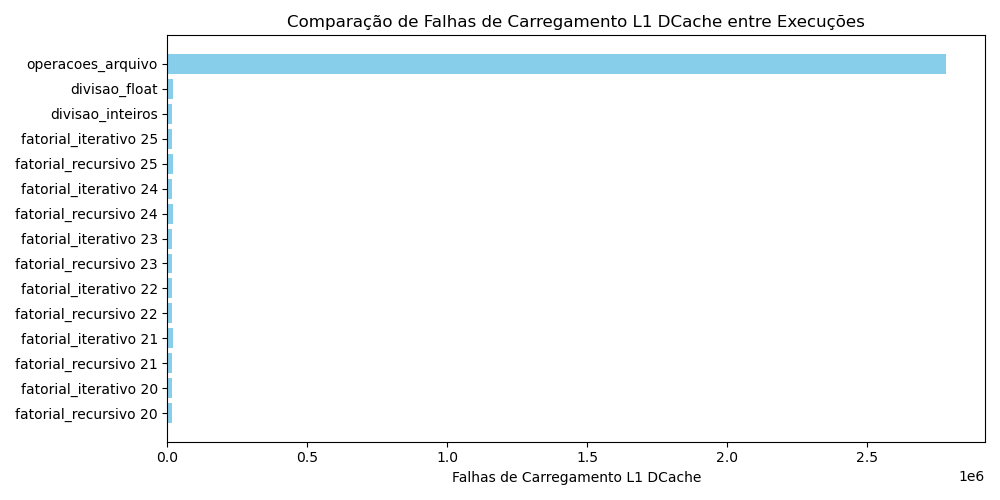
\includegraphics[width=\linewidth]{resultados/l1_dcache_load_misses.png}
    \caption{L1 DCache Load Misses dos Algoritmos}
    \label{fig:l1_dcache_load_misses}
\end{figure}

\begin{figure}[H]
    \centering
    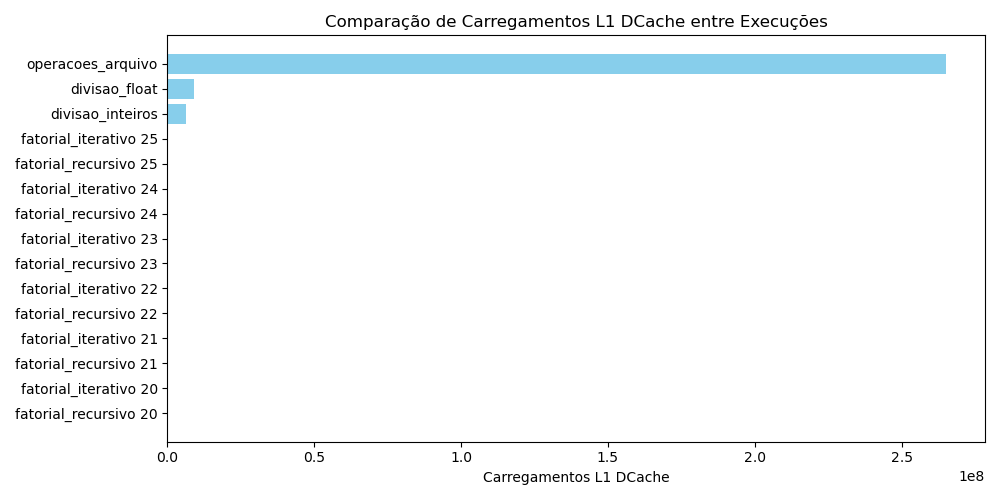
\includegraphics[width=\linewidth]{resultados/l1_dcache_loads.png}
    \caption{L1 DCache Loads dos Algoritmos}
    \label{fig:l1_dcache_loads}
\end{figure}

\begin{figure}[H]
    \centering
    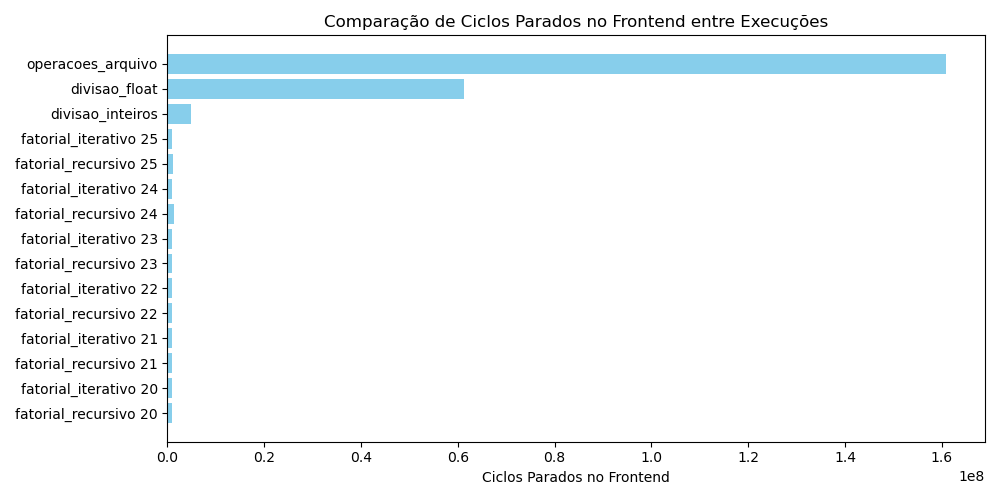
\includegraphics[width=\linewidth]{resultados/stalled_cycles_frontend.png}
    \caption{Stalled Cycles Frontend dos Algoritmos}
    \label{fig:stalled_cycles_frontend}
\end{figure}

\begin{figure}[H]
    \centering
    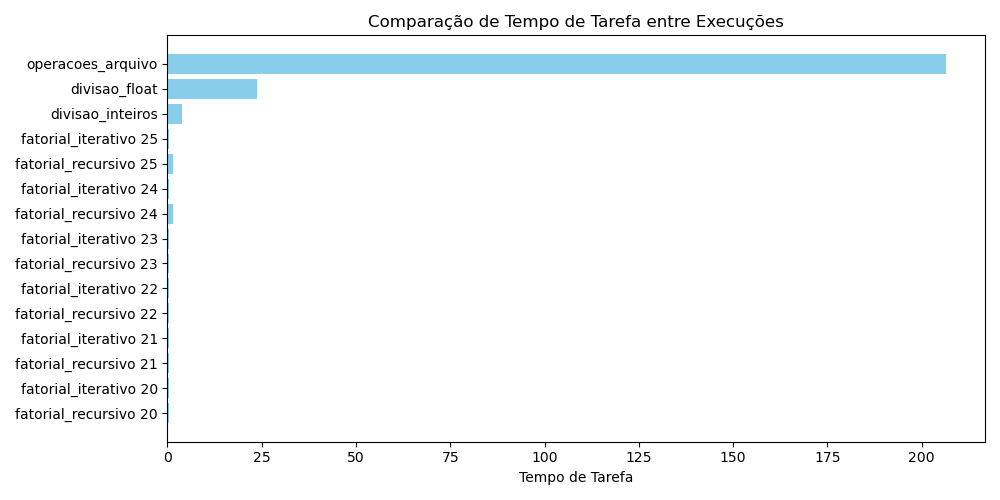
\includegraphics[width=\linewidth]{resultados/task_clock.png}
    \caption{Task Clock dos Algoritmos}
    \label{fig:task_clock}
\end{figure}

Os resultados mostram que o algoritmo iterativo tem um desempenho melhor em termos de tempo de execução e ciclos de CPU quando comparado ao algoritmo recursivo. As operações de divisão de inteiros e floats apresentaram desempenho similar, enquanto a operação de escrita em arquivo adicionou um overhead significativo devido ao I/O. A análise detalhada das métricas forneceu uma visão abrangente do comportamento dos algoritmos.

\section{Análise das Métricas}

Nesta seção, apresentamos as métricas de desempenho detalhadas para diferentes algoritmos e entradas. Cada métrica é explicada abaixo com suas respectivas fórmulas:

\begin{itemize}
    \item \textbf{Percentual do Tempo Total Gasto pela CPU}: Representa a porcentagem do tempo total de execução que a CPU utilizou para processar o algoritmo. É calculado como:
    \begin{equation}
    \text{Percentual do Tempo CPU} = \frac{\text{Tempo de Usuário} + \text{Tempo de Sistema}}{\text{Tempo Real}}
    \end{equation}

    \item \textbf{MIPS (Milhões de Instruções por Segundo)}: Mede o número de instruções executadas pela CPU por segundo. É calculado como:
    \begin{equation}
    \text{MIPS} = \frac{\text{Número de Instruções}}{\text{Tempo de CPU} \times 10^6}
    \end{equation}

    \item \textbf{MFLOPS (Milhões de Operações de Ponto Flutuante por Segundo)}: Mede o número de operações de ponto flutuante executadas pela CPU por segundo. É calculado como:
    \begin{equation}
    \text{MFLOPS} = \frac{\text{Número de Operações de Ponto Flutuante}}{\text{Tempo de CPU} \times 10^6}
    \end{equation}

    \item \textbf{Tempo de CPU}: Tempo total de uso da CPU para executar o algoritmo, calculado com base no número de ciclos de clock e a frequência do clock:
    \begin{equation}
    \text{Tempo de CPU} = \frac{\text{Número de Ciclos de Clock}}{\text{Frequência do Clock}}
    \end{equation}

    \item \textbf{Performance}: Uma medida geral de desempenho, calculada como o inverso do tempo de execução:
    \begin{equation}
    \text{Performance} = \frac{1}{\text{Tempo de Execução}}
    \end{equation}
\end{itemize}

\subsection{Métricas Detalhadas}

Também obtidas pelo plot.py

\begin{itemize}
    \item \textbf{Métricas para fatorial\_recursivo 10}:
    \begin{itemize}
        \item Percentual do tempo total gasto pela CPU: 1.07
        \item MIPS: 328.94
        \item MFLOPS: 475.06
        \item Tempo de CPU: 0.000585 segundos
        \item Performance: 510.041701
    \end{itemize}

    \item \textbf{Métricas para fatorial\_iterativo 10}:
    \begin{itemize}
        \item Percentual do tempo total gasto pela CPU: 1.19
        \item MIPS: 282.64
        \item MFLOPS: 400.00
        \item Tempo de CPU: 0.000618 segundos
        \item Performance: 477.432027
    \end{itemize}

    \item \textbf{Métricas para fatorial\_recursivo 20}:
    \begin{itemize}
        \item Percentual do tempo total gasto pela CPU: 0.61
        \item MIPS: 289.25
        \item MFLOPS: 410.68
        \item Tempo de CPU: 0.000677 segundos
        \item Performance: 249.671869
    \end{itemize}

    \item \textbf{Métricas para fatorial\_iterativo 20}:
    \begin{itemize}
        \item Percentual do tempo total gasto pela CPU: 1.48
        \item MIPS: 278.49
        \item MFLOPS: 391.85
        \item Tempo de CPU: 0.000690 segundos
        \item Performance: 578.603921
    \end{itemize}

    \item \textbf{Métricas para fatorial\_recursivo 30}:
    \begin{itemize}
        \item Percentual do tempo total gasto pela CPU: 0.19
        \item MIPS: 2995.12
        \item MFLOPS: 4166.67
        \item Tempo de CPU: 0.000603 segundos
        \item Performance: 774.745167
    \end{itemize}

    \item \textbf{Métricas para fatorial\_iterativo 30}:
    \begin{itemize}
        \item Percentual do tempo total gasto pela CPU: 0.97
        \item MIPS: 513.58
        \item MFLOPS: 714.29
        \item Tempo de CPU: 0.000643 segundos
        \item Performance: 695.476067
    \end{itemize}

    \item \textbf{Métricas para fatorial\_recursivo 40}:
    \begin{itemize}
        \item Percentual do tempo total gasto pela CPU: 1.14
        \item MIPS: 523.93
        \item MFLOPS: 688.71
        \item Tempo de CPU: 0.000625 segundos
        \item Performance: 781.710476
    \end{itemize}

    \item \textbf{Métricas para fatorial\_iterativo 40}:
    \begin{itemize}
        \item Percentual do tempo total gasto pela CPU: 1.12
        \item MIPS: 512.61
        \item MFLOPS: 676.59
        \item Tempo de CPU: 0.000642 segundos
        \item Performance: 759.330271
    \end{itemize}

    \item \textbf{Métricas para fatorial\_recursivo 50}:
    \begin{itemize}
        \item Percentual do tempo total gasto pela CPU: 1.15
        \item MIPS: 503.98
        \item MFLOPS: 634.92
        \item Tempo de CPU: 0.000664 segundos
        \item Performance: 728.938949
    \end{itemize}

    \item \textbf{Métricas para fatorial\_iterativo 50}:
    \begin{itemize}
        \item Percentual do tempo total gasto pela CPU: 0.94
        \item MIPS: 506.31
        \item MFLOPS: 645.16
        \item Tempo de CPU: 0.000688 segundos
        \item Performance: 606.211975
    \end{itemize}

    \item \textbf{Métricas para fatorial\_recursivo 60}:
    \begin{itemize}
        \item Percentual do tempo total gasto pela CPU: 1.10
        \item MIPS: 463.51
        \item MFLOPS: 555.86
        \item Tempo de CPU: 0.000781 segundos
        \item Performance: 610.654579
    \end{itemize}

    \item \textbf{Métricas para fatorial\_iterativo 60}:
    \begin{itemize}
        \item Percentual do tempo total gasto pela CPU: 0.18
        \item MIPS: 3214.19
        \item MFLOPS: 3875.97
        \item Tempo de CPU: 0.000681 segundos
        \item Performance: 682.795666
    \end{itemize}

    \item \textbf{Métricas para fatorial\_recursivo 70}:
    \begin{itemize}
        \item Percentual do tempo total gasto pela CPU: 1.13
        \item MIPS: 659.18
        \item MFLOPS: 745.71
        \item Tempo de CPU: 0.000631 segundos
        \item Performance: 844.712312
    \end{itemize}

    \item \textbf{Métricas para fatorial\_iterativo 70}:
    \begin{itemize}
        \item Percentual do tempo total gasto pela CPU: 1.10
        \item MIPS: 492.04
        \item MFLOPS: 553.10
        \item Tempo de CPU: 0.000864 segundos
        \item Performance: 611.065044
    \end{itemize}

    \item \textbf{Métricas para fatorial\_recursivo 80}:
    \begin{itemize}
        \item Percentual do tempo total gasto pela CPU: 1.14
        \item MIPS: 483.83
        \item MFLOPS: 505.05
        \item Tempo de CPU: 0.000808 segundos
        \item Performance: 573.493476
    \end{itemize}

    \item \textbf{Métricas para fatorial\_iterativo 80}:
    \begin{itemize}
        \item Percentual do tempo total gasto pela CPU: 1.03
        \item MIPS: 503.15
        \item MFLOPS: 533.90
        \item Tempo de CPU: 0.000878 segundos
        \item Performance: 549.992383
    \end{itemize}

    \item \textbf{Métricas para fatorial\_recursivo 90}:
    \begin{itemize}
        \item Percentual do tempo total gasto pela CPU: 0.98
        \item MIPS: 591.03
        \item MFLOPS: 583.43
        \item Tempo de CPU: 0.000797 segundos
        \item Performance: 573.065903
    \end{itemize}

    \item \textbf{Métricas para fatorial\_iterativo 90}:
    \begin{itemize}
        \item Percentual do tempo total gasto pela CPU: 0.17
        \item MIPS: 3672.06
        \item MFLOPS: 3623.19
        \item Tempo de CPU: 0.000854 segundos
        \item Performance: 607.870217
    \end{itemize}

    \item \textbf{Métricas para fatorial\_recursivo 100}:
    \begin{itemize}
        \item Percentual do tempo total gasto pela CPU: 1.15
        \item MIPS: 595.57
        \item MFLOPS: 545.55
        \item Tempo de CPU: 0.000809 segundos
        \item Performance: 625.671815
    \end{itemize}

    \item \textbf{Métricas para fatorial\_iterativo 100}:
    \begin{itemize}
        \item Percentual do tempo total gasto pela CPU: 0.58
        \item MIPS: 1196.09
        \item MFLOPS: 1096.49
        \item Tempo de CPU: 0.000785 segundos
        \item Performance: 631.041831
    \end{itemize}

    \item \textbf{Métricas para divisao\_inteiros}:
    \begin{itemize}
        \item Percentual do tempo total gasto pela CPU: 0.85
        \item MIPS: 4265.53
        \item MFLOPS: 160.49
        \item Tempo de CPU: 0.005984 segundos
        \item Performance: 136.773927
    \end{itemize}

    \item \textbf{Métricas para divisao\_float}:
    \begin{itemize}
        \item Percentual do tempo total gasto pela CPU: 0.82
        \item MIPS: 832.82
        \item MFLOPS: 38.69
        \item Tempo de CPU: 0.031143 segundos
        \item Performance: 31.678046
    \end{itemize}

    \item \textbf{Métricas para operacoes\_arquivo}:
    \begin{itemize}
        \item Percentual do tempo total gasto pela CPU: 1.00
        \item MIPS: 4002.54
        \item MFLOPS: 3.27
        \item Tempo de CPU: 0.242996 segundos
        \item Performance: 3.268903
    \end{itemize}
\end{itemize}

\newpage

\section{Conclusão}
A análise de desempenho realizada revelou que, para o cálculo do fatorial de números relativamente grandes, o método iterativo tende a ser menos discrepante em termos de tempo de execução e uso de ciclos de CPU. As operações de divisão mostraram-se eficientes, enquanto as operações de escrita em arquivo apresentaram maior overhead devido ao I/O. A ferramenta \textit{perf} foi essencial para coletar métricas detalhadas de desempenho, possibilitando uma análise mais aprofundada do que o \textit{time}. Tanto no VirtualBox quanto no Docker, a diferença entre as execuções não foi muito visível nos algoritmos de fatorial, mas nos algoritmos de divisão e, principalmente, de escrita em arquivo, o resultado foi notável.

\end{document}